%%%%%%%%%%%%%%%%%%%%%%%%%%%%%%%%%%%%%%%%%%%%%%%%%%%%%%%%%%%%%%%
%%%  notify DTS and PTS
%%%%%%%%%%%%%%%%%%%%%%%%%%%%%%%%%%%%%%%%%%%%%%%%%%%%%%%%%%%%%%%

\documentclass[onecolumn,fleqn]{revtex4}

% fonts
\usepackage{latexsym}
\usepackage{amsmath} 
\usepackage{amssymb} 
\usepackage{bm}
\usepackage{wasysym}

\usepackage{graphicx}

\usepackage{color}



% extra by jarondl
\usepackage{array}
%\usepackage{multicol}
\usepackage[caption=false]{subfig} %subcaption is not compat with revtex
\usepackage{verbatim}
\usepackage{environ}
\usepackage{etoolbox}
  \newbool{showfigure}
  \setbool{showfigure}{true}
  
\usepackage{enumerate}
  
\usepackage[pdftitle={PTA},bookmarks]{hyperref}


%%%%%%%%%%%%%%%%%%%%%%%%%%%%%%%%%%%%%%%%%%%%%%%%%%%%%%%%%%%%%%%%

% NEW 
\newcommand{\abs}[1]{\left|#1\right|}
\newcommand{\varphiJ}{\bm{\varphi}}
\newcommand{\thetaJ}{\bm{\theta}}
%\renewcommand{\includegraphics}[2][0]{FIGURE}
\newcommand{\rmrk}[1]{\textcolor{red}{#1}}
\newcommand{\Eq}[1]{\textcolor{blue}{Eq.\!\!~(\ref{#1})}} 
\newcommand{\Fig}[1]{\textcolor{blue}{Fig.}\!\!~\ref{#1}}

% math symbols I
\newcommand{\sinc}{\mbox{sinc}}
\newcommand{\const}{\mbox{const}}
\newcommand{\trc}{\mbox{trace}}
\newcommand{\intt}{\int\!\!\!\!\int }
\newcommand{\ointt}{\int\!\!\!\!\int\!\!\!\!\!\circ\ }
\newcommand{\ar}{\mathsf r}
\newcommand{\im}{\mbox{Im}}
\newcommand{\re}{\mbox{Re}}

% math symbols II
\newcommand{\eexp}{\mbox{e}^}
\newcommand{\bra}{\left\langle}
\newcommand{\ket}{\right\rangle}

% Mass symbol
\newcommand{\mass}{\mathsf{m}} 
\newcommand{\rdisc}{\epsilon} 

% more math commands
\newcommand{\tbox}[1]{\mbox{\tiny #1}}
\newcommand{\bmsf}[1]{\bm{\mathsf{#1}}} 
\newcommand{\amatrix}[1]{\begin{matrix} #1 \end{matrix}} 
\newcommand{\pd}[2]{\frac{\partial #1}{\partial #2}}

% equations
\newcommand{\mylabel}[1]{\label{#1}} 
\newcommand{\beq}{\begin{eqnarray}}
\newcommand{\eeq}{\end{eqnarray}} 
\newcommand{\be}[1]{\begin{eqnarray}\ifthenelse{#1=-1}{\nonumber}{\ifthenelse{#1=0}{}{\mylabel{e#1}}}}
\newcommand{\ee}{\end{eqnarray}} 

% arrangement
\newcommand{\hide}[1]{}
\newcommand{\drawline}{\begin{picture}(500,1)\line(1,0){500}\end{picture}}
\newcommand{\bitem}{$\bullet$ \ \ \ }
\newcommand{\Cn}[1]{\begin{center} #1 \end{center}}
\newcommand{\mpg}[2][1.0\hsize]{\begin{minipage}[b]{#1}{#2}\end{minipage}}
\newcommand{\mpgt}[2][1.0\hsize]{\begin{minipage}[t]{#1}{#2}\end{minipage}}

%%%%%%%%%%%%%%%%%%%%%%%%%%%%%%%%%%%%%%%%%%%%%%%%%%%%%%%%%%%%%%%%%%%%%%%%%%%
% Sections
\newcommand{\sect}[1]
{
\addtocounter{section}{1} 
\setcounter{subsection}{0}
\ \\ 
\pdfbookmark[2]{\thesection. \ #1}{sect.\thesection}
{\Large\bf $=\!=\!=\!=\!=\!=\;$ [\thesection] \ #1}  
\nopagebreak
}

% subections
\newcommand{\subsect}[1]
{
\addtocounter{subsection}{1} 
\ \\ 
\pdfbookmark[2]{\ \ \ \ \thesection.\thesubsection. \ #1}{subsect.\thesection.\thesubsection}
{\bf $=\!=\!=\!=\!=\!=\;$ [\thesection.\thesubsection] \ #1}  
\nopagebreak
}
%%%%%%%%%%%%%%%%%%%%%%%%%%%%%%%%%%%%%%%%%%%%%%%%%%%%%%%%%%%%%%%%%%%%%%%%
%%%%%%%%%%%%%%%%%%%%%%%%%%%%%%%%%%%%%%%%%%%%%%%%%%%%%%%%%%%%%

%%%%%%%%%%%%%%%%%%%%%%%%%%%% MESSING WITH DEFINITIONS
\newcommand{\chapter}[1]{}
%\RenewDocumentCommand {figure} { { v } }{\comment }{ \endcomment }
%\BeforeBeginEnvironment{figure}{\comment}
%\AfterEndEnvironment{figure}{\endcomment}

%\renewenvironment{figure}
%               {\expandafter\comment   hhh}
%               {\expandafter\endcomment      hhh  }
%\newenvironment{subfigure}[1]
%               {\hspace{1in}}
%               {}
%\renewenvironment{caption}[1]
%               {}
%               {}
\NewEnviron{subfigure}{{Ignore this.}}
%\RenewEnviron{caption}{}
\renewcommand{\caption}{}
\renewcommand{\subref}[1]{{}}

\graphicspath{{figures/}}
\begin{document}

\title{PTA}

\author{YdL}

%\maketitle

%%%%%%%%%%%%%%%%%%%%%%%%%%%%%%%%%%%%%%%%%%%%%%%%%%%%%%%%%%%%%%%%%%%%%%%%
%%%%%%%%%%%%%%%%%%%%%%%%%%%%%%%%%%%%%%%%%%%%%%%%%%%%%%%%%%%%%%%%%%%%%%%%

\rmrk{Here follows the segments completed work and
preliminary analysis, only with a ``notes'' like format}.


\chapter{Completed Work}


This work was published at Physical Review E \cite{de_leeuw_diffusion_2012},
and reprinted here in \autoref{sec:papers}. In the
following sections we will provide an overview
of the main results.


%%%%%%%%%%%%%%   Overview over article should not include too much equations
%%  bottom line - take home message - the derivations should ref the article

%%  
%%  remove the techinalities - 
%%     using the procedure we have calculated for.. blah blah
%%       see figure. (leave plots only if neccessary to buttom line).
%%
%%  geometry plots - maybe try with normal scale.
%%                   if that doesn't work, leave the figure out.



%%%%%%%%%%%%%%%%%%%%%%%%%

%%%%%%%%%%%%%
%\section{Article abstract}
%\rmrk{This is the article abstract..}


We have studied random networks whose dynamics are
described by a rate equation, with transition rates $w_{nm}$
that form a symmetric matrix (\autoref{sec:matrices}),
with a diagonal conforming to \autoref{eq:zero_sum}. 
%
The long time evolution
of the system is characterized by a diffusion coefficient~$D$.
In one dimension it is well known that $D$ can display an abrupt
percolation-like transition from diffusion (${D>0}$)
to sub-diffusion (${D=0}$). 
%
A question arises whether
such a transition happens in higher dimensions.
Numerically $D$ can be evaluated using a resistor network
calculation, or optionally it can be deduced from 
the spectral properties of the system. Contrary to a recent 
expectation that is based on a renormalization-group analysis, 
we deduce that $D$ is finite.
%
We suggest an ``effective-range-hopping'' procedure to evaluate $D$,
and contrast the results with the linear estimate.
The same approach is useful for the analysis of 
networks that are described by quasi-one-dimensional  
sparse banded matrices. 


%%%%%%%%%%%%%%%%%%%%%%%%%
\section{The effective range hopping procedure}


The basic idea behind \emph{ERH} (effective range hopping) is that in the linear
expression, nearby sites 
with $r\ll 1$ (and therefore $w \gg 1$ ) are over represented in
the diffusion coefficient calculation. While the transition to
these sites is indeed high, the distance covered is not enough
to form a percolating cluster. Therefore, we use a threshold based
on percolation theory and flat-down the rates higher then this threshold.
This produces a smooth crossover between the linear
estimate and the \emph{VRH} estimate.


Using the \emph{ERH} procedure we have calculated the diffusion for several models.


For the degenerate hopping model we obtained:

\begin{align}
D_{\tbox{ERH}} &=  \mathrm{EXP}_{d{+}2}\left(\frac{1}{s_c}\right)  \  \eexp{-1/s_c}  \ D_{\tbox{linear}}
\end{align}
%
For infinite dimensions ($d\rightarrow\infty$),  we have $\mathrm{EXP}_{d{+}2}\  \eexp{-1/s_c} = 1$. 
This means that the ERH expression converges with the linear expression.
For low dimensionality, the exponent dominant.


For the Mott Hopping model,
%
\begin{align}
D_{\tbox{ERH}} &=\mathrm{EXP}_{d{+}3}\left(\epsilon_c\right)  \  \eexp{-\epsilon_c}  \ D_{\tbox{linear}}
\end{align}
%


For the flat-profile banded $1d$ model,
\begin{align}
D_{\text{ERH}} \ \ &= \ \ 
\ \frac{1}{\sigma}\left[ 
\left(1+\frac{n_c}{2b}\sigma\right)\eexp{-\frac{n_c}{2b}\sigma} - \eexp{-2\sigma}
\right] \ \tilde{b} w_0 \\ &=\ \ 
\ \frac{\left(1+\frac{n_c}{2b}\sigma\right)\eexp{-\frac{n_c}{2b}\sigma} - \eexp{-2\sigma}}
       {1 - \eexp{-2\sigma}}
   \ D_{\tbox{linear}}
\end{align}



%%%%%%%%%%%%%%%%%%%%%%%%%%%%%%%%%%%%%%%%%%%%%%%%%%%%
%%%%%%%%%%%%%%%%%%%%%%%%%%%%%%%%%%%%%%%%%%%%%%%%%%%%
\chapter{Preliminary analysis}



%%%%%%%%%%%%%%%%%%%%%%%%%%%%%%%%%%%%%%%%%%%%%%%%%%%
%%%%   PTA                                    %%%%%
%%%%%%%%%%%%%%%%%%%%%%%%%%%%%%%%%%%%%%%%%%%%%%%%%%%
\section{Heat transport in sparse banded Hamiltonians}\label{sec:PTA}


We have analyzed a model of springs and masses described in \autoref{sec:app_heat}.
The Hamiltonian is quadratic in the $K$ matrix as defined in \autoref{eq:K_matrix},
which means that the eigenvalues $\lambda$ of $K$ determine the frequencies $\omega^2 = \lambda$.
The eigenmodes are of course the same. The analysis of this model in the resistor network perspective
and the lower-eigenvalues spectral analysis perspective is presented in the article, and we now
turn to inspect the heat transport angle.


As explained earlier, in contrast to the low-eigenvalue-only DC conductance, 
the total heat conductance is defined by the
sum over the heat conductances of the participating modes:
%
\begin{align}
G \ =\ \sum_n g(\lambda_n)
\end{align}
%
It is common to assume
that the temperature of the baths is high enough for all the modes to
participate, and for the bath spectrum to be white, meaning that all frequencies
have the same weight. The heat conductance of an eigenmode can be calculated
using the Landauer or the Kubo formalism, or, alternatively, can be estimated
via the PN (participation number), or the Thouless curvature. 
In recent studies \cite{bodyfelt_unpub} of \emph{pinned}\cite{roy_role_2008} banded matrices,
two groups of PN values were observed, and by counting the number of modes in the
higher PN group, the total conductance scaling was found. 



In \autoref{fig:pta} we have extended this analysis by studying the
effects of pinning, and by introducing sparsity. Also, we have
numerically calculated the Thouless conductance,
which we expect to correlate with $PN$. Disregarding major numerical issues,
the correlation seems to hold, see \autoref{fig:PN_g_scatter}.


As presented in \autoref{sec:heat}, the thermal conductance depends
on all the wide modes. The DC conductance, on the other hand,
depends on the $\lambda\rightarrow 0$ modes only. It seems that
for sparse systems these definitions coincide, since only 
the $\lambda\rightarrow 0$ modes are wide.


%%%%%%%%%%%%%%%%%%%%%%%%%%%%%%%%%%%%%%%%%%%%%%%%%%%%%%%%%%%%%%%%%%%%%%%%%%%%
%%  The following figure is displayed on rp.pdf but not on pta_dts_as_notes
%%     Because of the boolean showfigure.
%%%%%%%%%%%%%%%%%%%%%%%%%%%%%%%%%%%%%%%%%%%%%%%%%%%%%%%%%%%%%%%%%%%%%%%%%%%
\notbool{showfigure}{\begin{comment}}{}

\begin{figure}[H]
  %\subfloat[Low sparsity]{
  \begin{subfigure}{.45\linewidth}\centering
    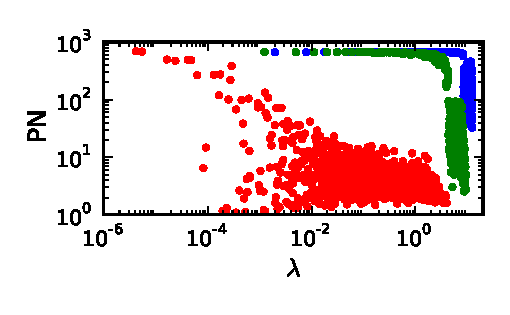
\includegraphics[width=0.99\linewidth]{pta_nopin}
    \caption{}\label{fig:PN_kottos_nopin}
  \end{subfigure}
  %
  \begin{subfigure}{.45\linewidth}\centering
     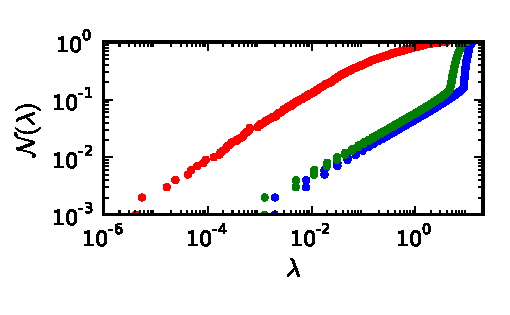
\includegraphics[width=0.99\linewidth]{pta_ev_nopin}
  \caption{}\label{fig:ev_dist}
  \end{subfigure}\\ % end of row
  %
 % \caption{}
 % \end{figure}
 % \begin{figure}[H]
  %
    \begin{subfigure}{.45\linewidth}\centering
    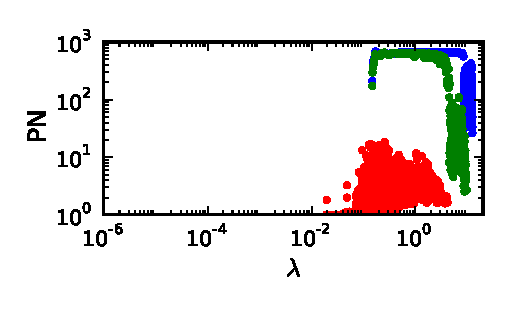
\includegraphics[width=0.99\linewidth]{pta_pin}
    \caption{}\label{fig:PN_kottos_pinning}
  \end{subfigure}     
  %
  \begin{subfigure}{.45\linewidth}\centering
     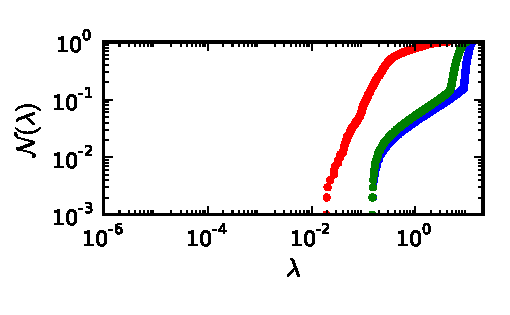
\includegraphics[width=0.99\linewidth]{pta_ev_pin}
  \caption{}\label{fig:ev_dist_pin}
  \end{subfigure}
    \begin{subfigure}{.45\linewidth}\centering
    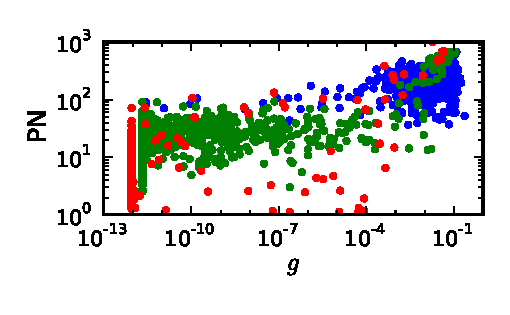
\includegraphics{pta_scatter_g}
  \caption{}\label{fig:PN_g_scatter}
  \end{subfigure}
  \caption{For all the plots $N=1000$ and $b=5$. 
           In blue $\sigma=0.1$, green $\sigma=0.6$ and red $\sigma=10$, where higher
           $\sigma$ means more sparsity.
           %%%%
           In (\subref{fig:PN_kottos_nopin}) with low $\sigma$ (blue) we see two groups of PN values.
           This distinction is lost for higher $\sigma$ (red).
           %%
           In (\subref{fig:ev_dist}) we plot the cumulative distribution of
           the eigenvalues, presenting clear diffusive behavior, for any $\sigma$.
           %%%%%% pinning
           In (\subref{fig:PN_kottos_pinning}) and (\subref{fig:ev_dist})
           we see the effects of diagonal disorder (pinning)
           on the spectrum. We see clearly that the lowest eigenvalues 
           are affected, and their corresponding PN is much lower. The spectrum
           reveals sub-diffusive behavior.
           %%%g 
           In (\subref{fig:PN_g_scatter}) we compare the Thouless conductance
           $g$ with the participation number. 
           The presented points do seem to be correlated, but due to numerical issues,
           many values of $g$ are below the precision limit (seen as a vertical line in the plot), 
           up to $936$ from $1000$ for $\sigma=10$. 
  }\label{fig:pta}
\end{figure}

\notbool{showfigure}{\end{comment}}{}




%%%%%%%%%%%%%%%%%%%%%%%%%%%%%%%%%%%%%%%%%%%%%%%%%%%%%%%%%
%%%%%%%%%   DTS
%%%%%%%%%%%%%%%%%%%%%%%%%%%%%%%%%%%%%%%%%%%%%%%%%%%%%%%%%

%%%%%%%%%%%%%%%%%%%%%%%%%%%%%
\section{Quantum spreading in a sparse banded Hamiltonian}\label{sec:dts}

In this section the numerical work was done by our collaborators,
Eli Halperin and Tsampikos Kottos of Wesleyan university.


We define a Hamiltonian
\begin{align}
\mathcal{H}\ \ &=\ \ \epsilon B_{nm}\\
B_{nm} \ \ &= \ \ \textrm{random}[\pm]\eexp{-x}\qquad 0<|n-m| \le b \\
x \ \ &= \ \ \textrm{random} \ \in [0,\sigma]
\end{align}
that depends on three parameters, $\epsilon$, $b$ and $\sigma$. The $\sigma$
parameter controls the sparsity, and $b$ is the bandwidth, and $\epsilon$
defines the units of frequency.
In past works \cite{cohen_wave_2000,stotland_random-matrix_2010} it was deduced that the diffusion coefficient 
in a disordered banded system can be calculated as:
\begin{align}
D_0 \ \ &=\ \ \left[b\ \textrm{Var}[B_{nm}]\right]^{1/2}\ b^2\epsilon \\
\textrm{VAR}(B_{nm}) \ \ &=\ \ \int_0^\sigma \left(\pm \eexp{-x}\right)^2 \frac{dx}{\sigma}\ \ 
 =\ \  \frac{1-\eexp{-2\sigma}}{2\sigma} \\
 D_0\ \ &\propto\ \ b^{2.5}\ \sqrt{\frac{1-\eexp{-2\sigma}}{2\sigma}} 
\end{align}

To question the validity of this result in the case of high sparsity,
we plot in \autoref{fig:D_of_s} the numerical results for $D$ divided by 
the speculated $D_0$. The results reveal that the sparsity affects the diffusion coefficient.
We see that as the system becomes more sparse, the diffusion coefficient is suppressed,
and as might be expected, the lower bandwidth ensembles are more
susceptible, as the system is more vulnerable to disconnections.


The next speculation is to use the suppression factor for sparse networks 
obtained in our previous work \autoref{sec:papers}:
%
\begin{align}
g_s(\sigma, b)\ \ &=\ \ \frac{D_{ERH}}{D_{\textrm{linear}}}\ \ =\ \ 
\frac{  \left(1+\frac{n_c}{b}\sigma\right)\eexp{-\frac{n_c}{b}\sigma}
                                              - \eexp{-4\sigma}}{1-\eexp{-4\sigma}}\\
\textrm{With } n_c\ &\approx 2
\end{align}

In \autoref{fig:d_vs_g} we plot a log-log scale, assuming a relation:
%
\begin{align}
\frac{D}{D_0}\ \ \approx \ \ C\ \ g_s(\sigma,b)^\gamma
\end{align}

From numerical fitting we see that $C\approx \frac{3}{4}$, 
and $\gamma$ is difficult to extract from this data set. We assume
that a wider range of $\sigma$ values will offer more knowledge.

\begin{figure}
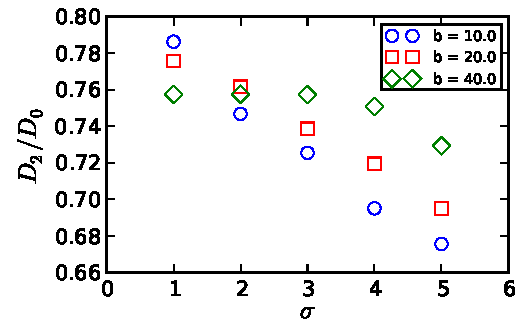
\includegraphics{dts_D2}
\caption{The transient diffusion coefficient for quantum spreading in
a banded sparse network. The ratio $D/D_0$ between the numerical diffusion 
coefficient and the expected value decreases as $\sigma$ increases. The effect
is stronger for low bandwidth.}\label{fig:D_of_s}
\end{figure}


\begin{figure}
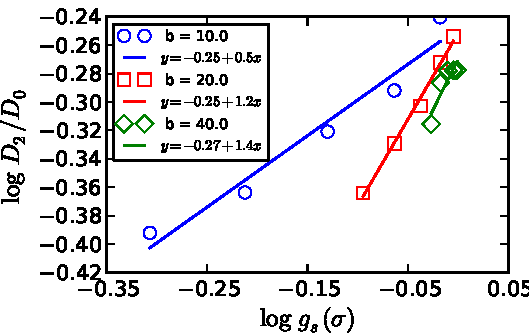
\includegraphics{dts_D2_vs_gs_loglog}
\caption{Scaled $D$ vs $g_s$. }\label{fig:d_vs_g}
\end{figure}


%\bibliographystyle{apsrev_doi}
\bibliographystyle{apsrev4-1}
%\nocite{revtex41Control}
\nocite{apsrev41Control}
\bibliography{jarondl,custom-longbib,manual_bib}

\end{document}
